\documentclass[12pt, a4paper]{article}% тип документа, размер шрифта
\usepackage[T2A]{fontenc}%поддержка кириллицы в ЛаТеХ
\usepackage[utf8]{inputenc}%кодировка
\usepackage[russian]{babel}%русский язык
\usepackage{mathtext}% русский текст в формулах
\usepackage{amsmath}%удобная вёрстка многострочных формул, масштабирующийся текст в формулах, формулы в рамках и др.
\usepackage{amsfonts}%поддержка ажурного и готического шрифтов — например, для записи символа {\displaystyle \mathbb {R} } \mathbb {R} 
\usepackage{amssymb}%amsfonts + несколько сотен дополнительных математических символов
\frenchspacing%запрет длинного пробела после точки
\usepackage{setspace}%возможность установки межстрочного интервала
\usepackage{indentfirst}%пакет позволяет делать в первом абзаце после заголовка абзацный отступ
\usepackage[unicode, pdftex]{hyperref}
\onehalfspacing%установка полуторного интервала по умолчанию
\usepackage{graphicx}%подключение рисунков
\graphicspath{{images/}}%путь ко всем рисункам
\usepackage{caption}
\usepackage{float}%плавающие картинки
\usepackage{tikz} % это для чудо-миллиметровки
\usepackage{pgfplots}%для построения графиков
\pgfplotsset{compat=newest, y label style={rotate=-90},  width=10 cm}%версия пакета построения графиков, ширина графиков
\usepackage{pgfplotstable}%простое рисование табличек
\usepackage{lastpage}%пакет нумерации страниц
\usepackage{comment}%возможность вставлять большие комменты
\usepackage{float}
%%%%% ПОЛЯъ
\setlength\parindent{0pt} 
\usepackage[top = 2 cm, bottom = 2 cm, left = 1.5 cm, right = 1.5 cm]{geometry}
\setlength\parindent{0pt}
%%%%% КОЛОНТИТУЛЫ
\usepackage{xcolor}
\usepackage{amsmath}
\usepackage{gensymb}
\usepackage{tikz}

\begin{document}

\subsubsection*{Первый закон Ньютона}
\textit{Инерциальная система отсчёта} — это такая система, в которой свободные тела (не подвергающиеся воздействию сил) движутся прямолинейно и равномерно. 


\textit{Первый закон Ньютона} утверждает, что существуют инерциальные системы отсчёта, то есть системы отсчёта, в которых тела сохраняют постоянную по модулю и направлению скорость, если на них не действуют внешние силы:
\[
\sum\vec F = 0 \quad\Longrightarrow\quad \vec v = \text{const}.
\]

\subsubsection*{Второй закон Ньютона}
Если на тело массы \(m\) действует результирующая сила \(\sum\vec F\), то за малый промежуток времени \(\Delta t\) изменение его скорости пропорционально этой силе:
\[
\sum\vec F = m\,\frac{\Delta\vec v}{\Delta t}.
\]
Вводя ускорение \(\vec a = \dfrac{\Delta\vec v}{\Delta t}\), получаем
\[
\sum\vec F = m\,\vec a.
\]

\textbf{Пример 1.}

На тело массой \(m\) действует сила тяжести \(\vec F_g = m\vec g\), 
где \(g\approx9.8\ \mathrm{м/с^2}\) — ускорение свободного падения. По второму закону Ньютона:
\[
m\vec a = m\vec g
\quad\Rightarrow\quad
\vec a = \vec g.
\]
Тело движется с ускорением \(g\) вниз.

\textbf{Пример 2.}

Рассмотрим блок массой \(m\) на шероховатой плоскости, наклонённой под углом \(\alpha\) к горизонту. 

\begin{center}
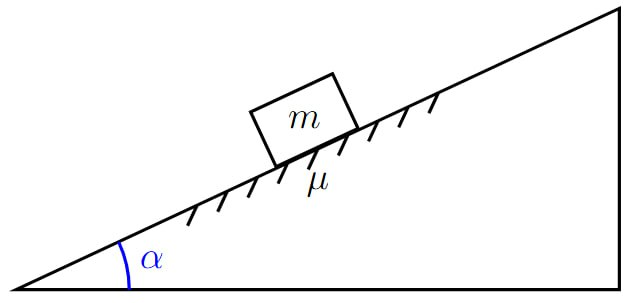
\includegraphics[width=0.43\linewidth]{9newton1.jpeg}
\label{fig:mpr}
\end{center}

Сила тяжести разлагается на:
\[
F_{g\,\parallel} = mg\sin\alpha
\quad\text{(вдоль плоскости)},\quad
F_{g\,\perp} = mg\cos\alpha
\quad\text{(перпендикулярно)}.
\]
Сила трения \(F_{\text{тр}}=\mu F_{g\,\perp}=\mu mg\cos\alpha\), направлена против движения. По второму закону вдоль плоскости:
\[
ma = mg\sin\alpha - \mu mg\cos\alpha
\quad\Rightarrow\quad
a = g\bigl(\sin\alpha - \mu\cos\alpha\bigr).
\]
Блок скатывается вниз с этим ускорением, если проекция силы тяжести пересиливает силу трения, то есть при

\[
\sin\alpha \geq \mu\cos\alpha
\]

\subsubsection*{Третий закон Ньютона}
Напомним, что третий закон Ньютона гласит, что любые два тела системы взаимодействуют с силами, равными по модулю и противоположными по направлению, направленными вдоль одной прямой:
\[
\vec F_{i\to j} = -\,\vec F_{j\to i}.
\]


\subsubsection*{Центр масс}
Для системы точек с массами $m_i$ и радиус-векторами $\vec r_i$ определим \textit{центр масс} $C$ так, чтобы его радиус-вектор (то есть вектор из центра координат до него) был равен
\[
\vec R_C = \frac{1}{M}\sum_i m_i\cdot\vec r_i,
\]
где \[M=\sum_i m_i.\]
За малый промежуток времени $\Delta t$ каждая точка сместилась на $\Delta\vec r_i$, тогда смещение центра масс
\[
\Delta\vec R_C = \frac{1}{M}\sum_i m_i\cdot\Delta\vec r_i.
\]
Делим на $\Delta t$:
\[
\frac{\Delta\vec R_C}{\Delta t} = \frac{1}{M}\sum_i m_i\cdot\frac{\Delta\vec r_i}{\Delta t}
\;\Longrightarrow\;
\vec V_C = \frac{1}{M}\sum_i m_i\vec v_i.
\]
То есть система движется так, как если бы вся масса $M$ была сосредоточена в точке $C$ со скоростью $\vec V_C$.



\subsubsection*{Теорема о движении центра масс}
Для системы частиц массами \(m_i\) под действием внешних сил
\(\vec F_i^{\mathrm{(ext)}}\) центр масс движется так, как если бы на него
действовала суммарная внешняя сила:
\[
M\vec a_C = \sum_i \vec F_i^{\mathrm{(ext)}}, 
\quad M=\sum_i m_i,
\]
где \(\vec a_C\) — ускорение центра масс.

Выведем теорему из законов Ньютона. 
Скорость центра масс \[\vec V_C = \frac1M\sum_i m_i\vec v_i.\]  


\begin{center}
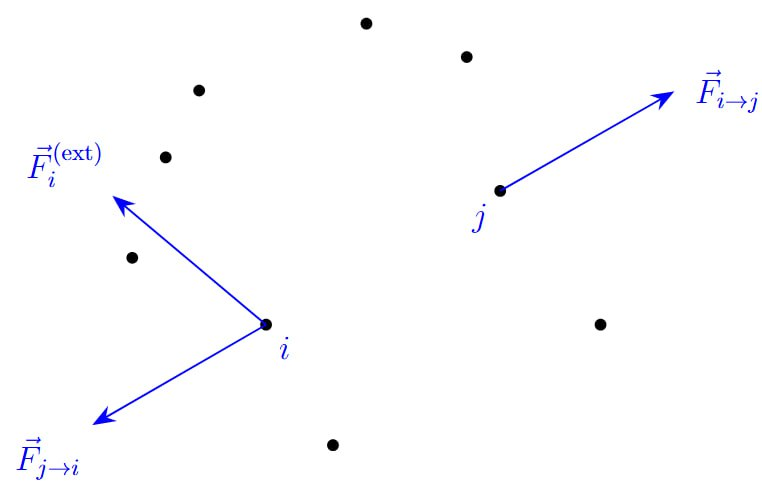
\includegraphics[width=0.53\linewidth]{9newton2.jpeg}
\label{fig:mpr}
\end{center}


По второму закону для каждой частицы \(i\):  
\[
m_i\,\frac{\Delta\vec v_i}{\Delta t}
= \vec F_i^{\mathrm{(ext)}} + \sum_{j\ne i}\vec F_{j\to i}.
\]
Складывая по всем \(i\):
\[
\sum_i m_i\,\frac{\Delta\vec v_i}{\Delta t}
= \sum_i \vec F_i^{\mathrm{(ext)}} 
+ \sum_{i}\sum_{j\ne i}\vec F_{j\to i}.
\]
По третьему закону второй двойной суммарный член равен нулю (внутренние силы взаимно
компенсируются). Получаем:
\[
M\vec a_C = M\,\frac{\Delta\vec V_C}{\Delta t}
= \sum_i \vec F_i^{\mathrm{(ext)}}.
\]


\end{document}